\begin{surferPage}[Septique heptagonale]{Une Septique à symétrie heptagonale}
    Cette surface ressemblant à une étoile est de degré $7$.
    Jusqu'à récemment, le nombre de ses singularités réelles, $84$,
    était le plus grand connu pour les Septiques;
    c'est seulement en 2004 qu'Oliver Labs a porté ce record à $99$.
  
  
 Les trois cocons que l'on peut voir sur l'image interactive 
    proviennent de l'utilisation des polynômes de Chebychev, de même que pour l'Octique de Chmutov.
    En fait, cette surface en forme d'étoile est une variante des surfaces de Chmutov.
    La courbe plane $T_d(x)+T_d(y)$ a ici été remplacée par un heptagone régulier
    $S_7(x,y)$: 
   \[S_7(x,y) + \lambda \cdot T_d(z) = 0,\]
    pour $\lambda\in\RR$ bien choisi. 
    \vspace*{-0.3em}
    \begin{center}
      \begin{tabular}{c@{\qquad}c}
        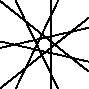
\includegraphics[height=1.5cm]{./../../common/images/labsseptic1.pdf}
        &
        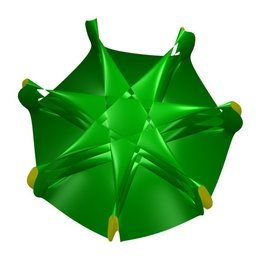
\includegraphics[height=1.5cm]{./../../common/images/septic_7eck_von_oben}
      \end{tabular}
    \end{center}
    \vspace*{-0.3em}   
   Cette variante de la construction de Chmutov est l'œuvre de Duco van Straten.
\end{surferPage}
